\section{Azure Stream Analytics}
Vor allem im heutigen Industrie 4.0 Umfeld sammeln sich schnell umfangreiche Datenmengen. Diese können oft nur über einen (stark) begrenzten Zeitraum zurückgehalten werden, da sie ansonsten ihre Aussagekraft verlieren. Ab diesem Punkt muss eine Datenverarbeitung erfolgen. Hier bietet Azure Stream Analytics eine Lösung. Dieser Dienst erlaubt Einblicke in Daten, um darin beispielsweise nach Mustern oder Anomalien zu suchen und entsprechend darauf zu reagieren \cite{Klein.2017}. Azure Stream Analytics unterstützt dabei eine SQL-Ähnliche Abfragesprache Stream Analytics Query Language (SAQL), über welche die dynamischen Datenströme analysiert werden. Obwohl SAQL von der allgegenwärtigen SQL-Abfragesprache abgeleitet wurde, enthält es Funktionen, die für die Stream-Verarbeitung notwendig sind \cite{Prosise.}. Eine dieser Funktionen ist die Möglichkeit, Ergebnisse mithilfe von Zeitfenstern zu erhalten (siehe Fensterfunktionen). Ein typisches Echtzeitverarbeitungssystem, welches auf Stream Analytics und weiteren Azure-Diensten aufbaut, ist in Abbildung \ref{uebersicht} aufgeführt.
\begin{figure*}[ht]
	\centering
	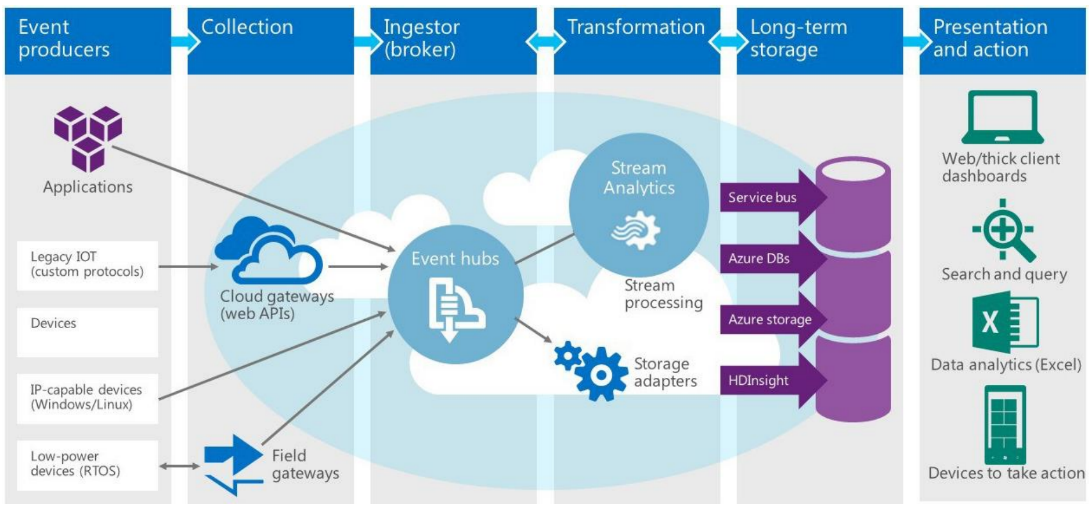
\includegraphics[width=0.8\textwidth,]{images/StreamAnalytics}
	\caption{Typisches Echtzeitverarbeitungssystem \cite{Prosise.}}
	\label{uebersicht}
\end{figure*}
\\ \\Die linke Spalte zeigt Sensoren, Geräte und andere Datenquellen einer IoT-Lösung. Diese senden permanent Daten über das Cloud Gateway an die Azure Hubs. Der Gateway-Dienst ist hierbei ein virtuelles Gerät und ermöglicht eine konsistente Verbindung. Die Hubs sind in der Lage Millionen von Ereignissen pro Sekunde zu verarbeiten. Von dort aus werden Ereignisse an weitere Anwendungen übergeben. Stream Analytics transformiert eingehenden Daten. Die Ausgaben lassen sich daraufhin auf eine Vielzahl von Endpunkten richten. Azure bietet hier einige Dienste, welche daran angeknüpft werden können \cite{Prosise.}. \\
Sowohl Ein- als auch Ausgaben, die ein Stream Analytics-Job benötigt, werden im Azure-Portal konfiguriert. Ein einzelner Stream Analytics-Job kann mehrere Eingaben enthalten. Durch Aggregation der Datenströme lassen sich kombinierte Abfragen durchführen. Dies kann mit einem JOIN in SQL verglichen werden. Dadurch, dass ein einzelner Stream Analytics-Job mit mehreren Ein- und Ausgängen konfiguriert werden kann, ermöglicht umfangreiche Topologien. Zur Verfügung stehen hier eine Reihe von Services (siehe  \cite{Prosise.})

\subsection{Fensterfunktionen}
Das Hauptfeature der Stream Analytics-Abfragesprache SAQL ist die Unterstützung von Fensterfunktionen. Nachfolgend werden die Funktionen aufgeführt \cite{Prosise.}: 
\begin{itemize} 
	\item TumblingWindow
	\item HoppingWindow
	\item SlidingWindow
\end{itemize}
Zeitfenster erlauben es für Datenströme temporale Vorgänge durchzuführen. Die Ausgabe eines Fensters ist ein einzelnes Ergebnis, welches auf der verwendeten Aggregatfunktion basiert (siehe \ref{fig:window_concepts}). 
\begin{figure}[H]
	\centering
	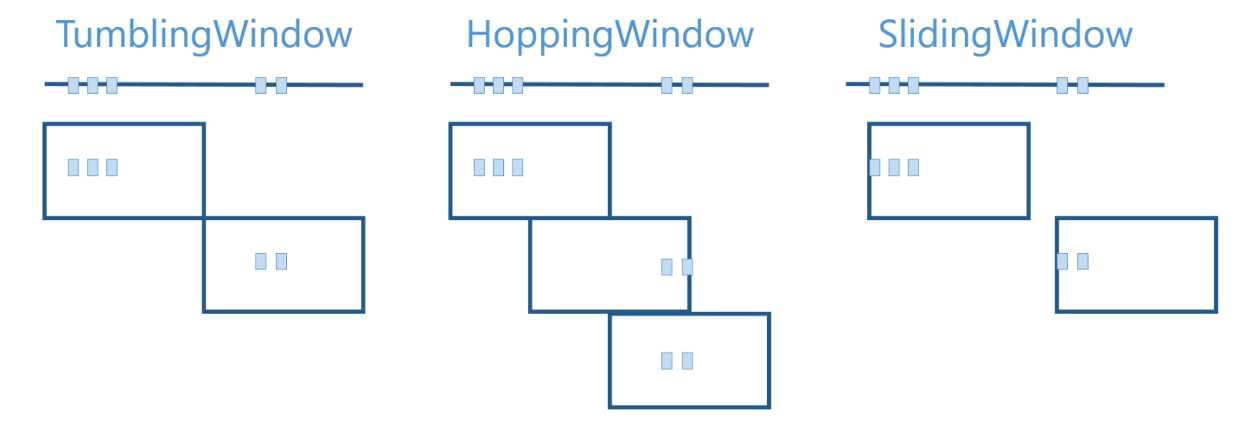
\includegraphics[width=1.0\linewidth]{images/fensterfunktionen}
	\caption{Fensterkonzepte \cite{Prosise.}} %Generelle
	\label{fig:window_concepts}
\end{figure} 
Das Resultat enthält einen Zeitstempel vom Ende des Fensters. Ein Fenster wird stets über eine feste Länge definiert. Alle Ergebnisse sollten mit einer GROUP BY-Klausel entsprechend zusammengeführt werden \cite{Azure.2017}. 
Als Exempel dient eine Aggregatfunktion, die aufzeigt, wie viele Autos einer speziellen Farbe alle fünf Minuten eine Mautstelle passieren \cite{Prosise.}. Mit TumblingWindow wird ein Datenstrom in einzelne Zeitsegmente unterteilt. Für diese unterteilten Segmente wird eine Funktion ausgeführt. Die Abfrage kann hier äquivalent zum oben beschriebenen Beispiel ausgedrückt werden. Bei den rollierenden Fenstern gibt es keine Überlappungen und ein Ergebnis kann nicht zu mehreren Fenstern gehören. Bei HoppingWindow wird immer für einen festen Zeitraum einen Sprung nach vorne durchgeführt. Grundsätzlich kann dieser Ansatz wie das TumblingWindow angesehen werden, bloß überlappen sich die wiederholenden Fenster. Durch diesen Umstand kann es sein, dass ein Ergebnis zu mehreren Fenstern gehören kann. Die Abfragen lassen sich ähnlich ausdrücken, allerdings kann hier unabhängig von der Fenstergröße eine Ausgabe erzeugt werden. Es lässt sich beispielsweise einmal pro Minute ausgegeben, wie viele Autos einer speziellen Farbe alle fünf Minuten diese Mautstelle anfahren. SlidingWindow hingegen erzeugt nur ein Ereignis, wenn entsprechende Anforderungen erfüllt sind \cite{Azure.2017}. Auch hier können Ergebnisse zu mehreren Fenstern gehören. Dieser Ansatz lässt die Abfrage zu, in welchen Fünf-Minuten-Zeitfenstern zehn oder mehr Autos einer speziellen Farbe die Mautstelle erreichen. SlidingWindow ist somit für den Umgang mit relativ spärlichen Ergebnismengen geeignet \cite{Prosise.}.

 